\documentclass[11pt]{article}
\usepackage[a4paper,margin=1in]{geometry}
\usepackage{graphicx}
\usepackage{booktabs}
\usepackage{longtable}
\usepackage{array}
\usepackage{hyperref}
\usepackage{amsmath}
\usepackage{amssymb}
\usepackage{siunitx}
\DeclareSIUnit\angstrom{\text{\AA}}
\usepackage{caption}
\usepackage{float}
\usepackage{enumitem}
\usepackage{xcolor}
\hypersetup{colorlinks=true,linkcolor=blue,urlcolor=blue,citecolor=blue}
\graphicspath{{figures/}}
\setlength{\parskip}{0.5em}
\setlength{\parindent}{0pt}

\title{PFAS Interfacial Package\\Technical Development and Reproducibility Report}
\author{Repository: \texttt{Prasanna163/PFAS-Interfacial-Package}}
\date{Generated on 2026-03-24}

\begin{document}
\maketitle
\tableofcontents
\newpage

\section{Executive Summary}
This report documents the current production codebase, its full workflow mechanics, and its development history up to commit \texttt{8787cbd} (2026-03-24). It is written as a reproducibility and handover document for re-running the PFAS interfacial study after data loss.

Core outcomes of this report are:
\begin{enumerate}[leftmargin=1.5em]
\item A complete technical walkthrough of the repository modules, CLI interfaces, data flow, and outputs.
\item A commit-level development timeline from initial package creation through \texttt{improvements-v1} and \texttt{V2} modularization.
\item Manuscript-aligned methodology mapping (including dual-orientation workflow and KNF context logic).
\item Sample calculations from manuscript-reported values, included in reproducible formula form.
\item A limitations and risk register focused on immediate reproducibility and next implementation priorities.
\end{enumerate}

\section{Repository Snapshot}
\subsection{Top-level Structure}
Current repository layout (main branch):
\begin{itemize}[leftmargin=1.5em]
\item \texttt{pfas\_interface\_cli/}: production Python package
\item \texttt{run\_pfas\_interface\_knf.py}: compatibility shim
\item \texttt{references/}: canonical slab files
\item \texttt{examples/}: sample slab files
\item \texttt{tools/}: utility scripts and analysis helpers
\item \texttt{docs/manuscript.pdf}: manuscript used as methodological basis
\end{itemize}

\subsection{Package Modules and Responsibilities}
\begin{table}[H]
\centering
\caption{Current modular architecture in \texttt{pfas\_interface\_cli}}
\begin{tabular}{p{0.23\textwidth}p{0.70\textwidth}}
\toprule
Module & Responsibility \\
\midrule
\texttt{cli.py} & User-facing command \texttt{PFAS}; default slab resolution; single-file and directory batch dispatch into workflow. \\
\texttt{workflow.py} & End-to-end orchestration: slab sort, xTB runs, orientation branches, KNF runs, analysis, report generation. \\
\texttt{geometry.py} & XYZ parsing/writing, bounds/centroid math, rotation matrix generation, slab O-H-H z-sorting. \\
\texttt{placement.py} & Head-tail axis inference, perpendicular/parallel orientation transform, slab-relative translation and merge. \\
\texttt{xtb.py} & xTB command execution and optimized energy parsing from \texttt{xtbopt.xyz}. \\
\texttt{knf.py} & KNF pipeline invocation on pre-optimized structures (no KNF-side geometry optimization). \\
\texttt{analysis.py} & Interface geometric diagnostics, closest-contact detection, KNF metric extraction and delta logic. \\
\texttt{reporting.py} & Human-readable summary table rendering and report text assembly. \\
\bottomrule
\end{tabular}
\end{table}

\begin{figure}[H]
\centering
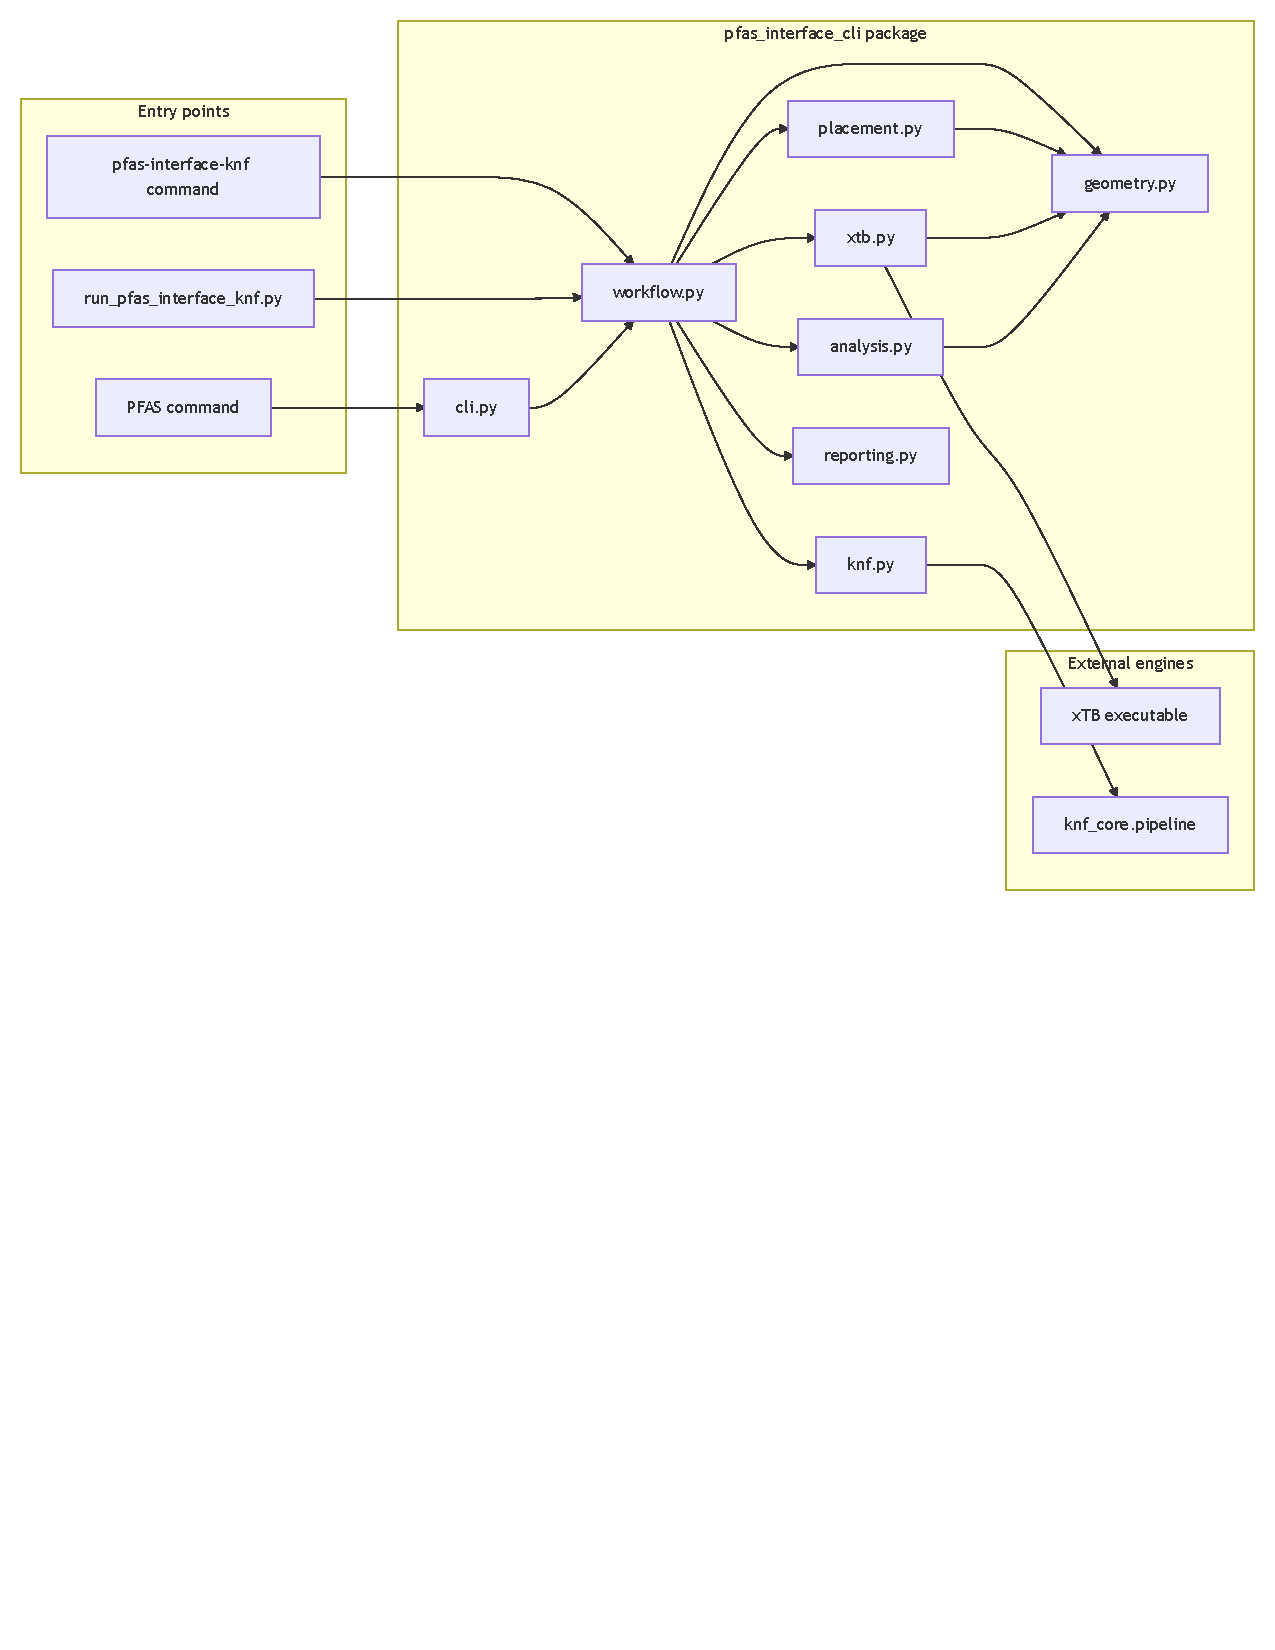
\includegraphics[width=\textwidth,height=0.75\textheight,keepaspectratio]{module_architecture.pdf}
\caption{Module dependency and external engine interfaces (Mermaid rendered to PDF).}
\end{figure}

\section{Development History and Change Log}
\subsection{Chronological Commit Timeline}
\begin{table}[H]
\centering
\caption{Main development milestones}
\begin{tabular}{p{0.16\textwidth}p{0.18\textwidth}p{0.60\textwidth}}
\toprule
Commit & Date & Summary \\
\midrule
\texttt{3e8a5ca} & 2026-03-03 & Initial commit (license scaffolding). \\
\texttt{9c3d150} & 2026-03-03 & Initial PFAS interfacial package with monolithic workflow script and helper scripts. \\
\texttt{698ee3a} & 2026-03-03 & Merge sync with remote main. \\
\texttt{5c1bdfa} & 2026-03-24 & Major refactor: dual-orientation pipeline, CLI workflow improvements, repository reorganization into \texttt{examples/}, \texttt{references/}, \texttt{tools/}. \\
\texttt{67b4c17} & 2026-03-24 & Merge of \texttt{improvements-v1} into \texttt{main}. \\
\texttt{38f3d3e} & 2026-03-24 & V2 modularization into \texttt{geometry}, \texttt{xtb}, \texttt{placement}, \texttt{analysis}, \texttt{reporting}, \texttt{workflow}, \texttt{knf}. \\
\texttt{8787cbd} & 2026-03-24 & Merge of \texttt{V2} into \texttt{main}. \\
\bottomrule
\end{tabular}
\end{table}

\begin{figure}[H]
\centering
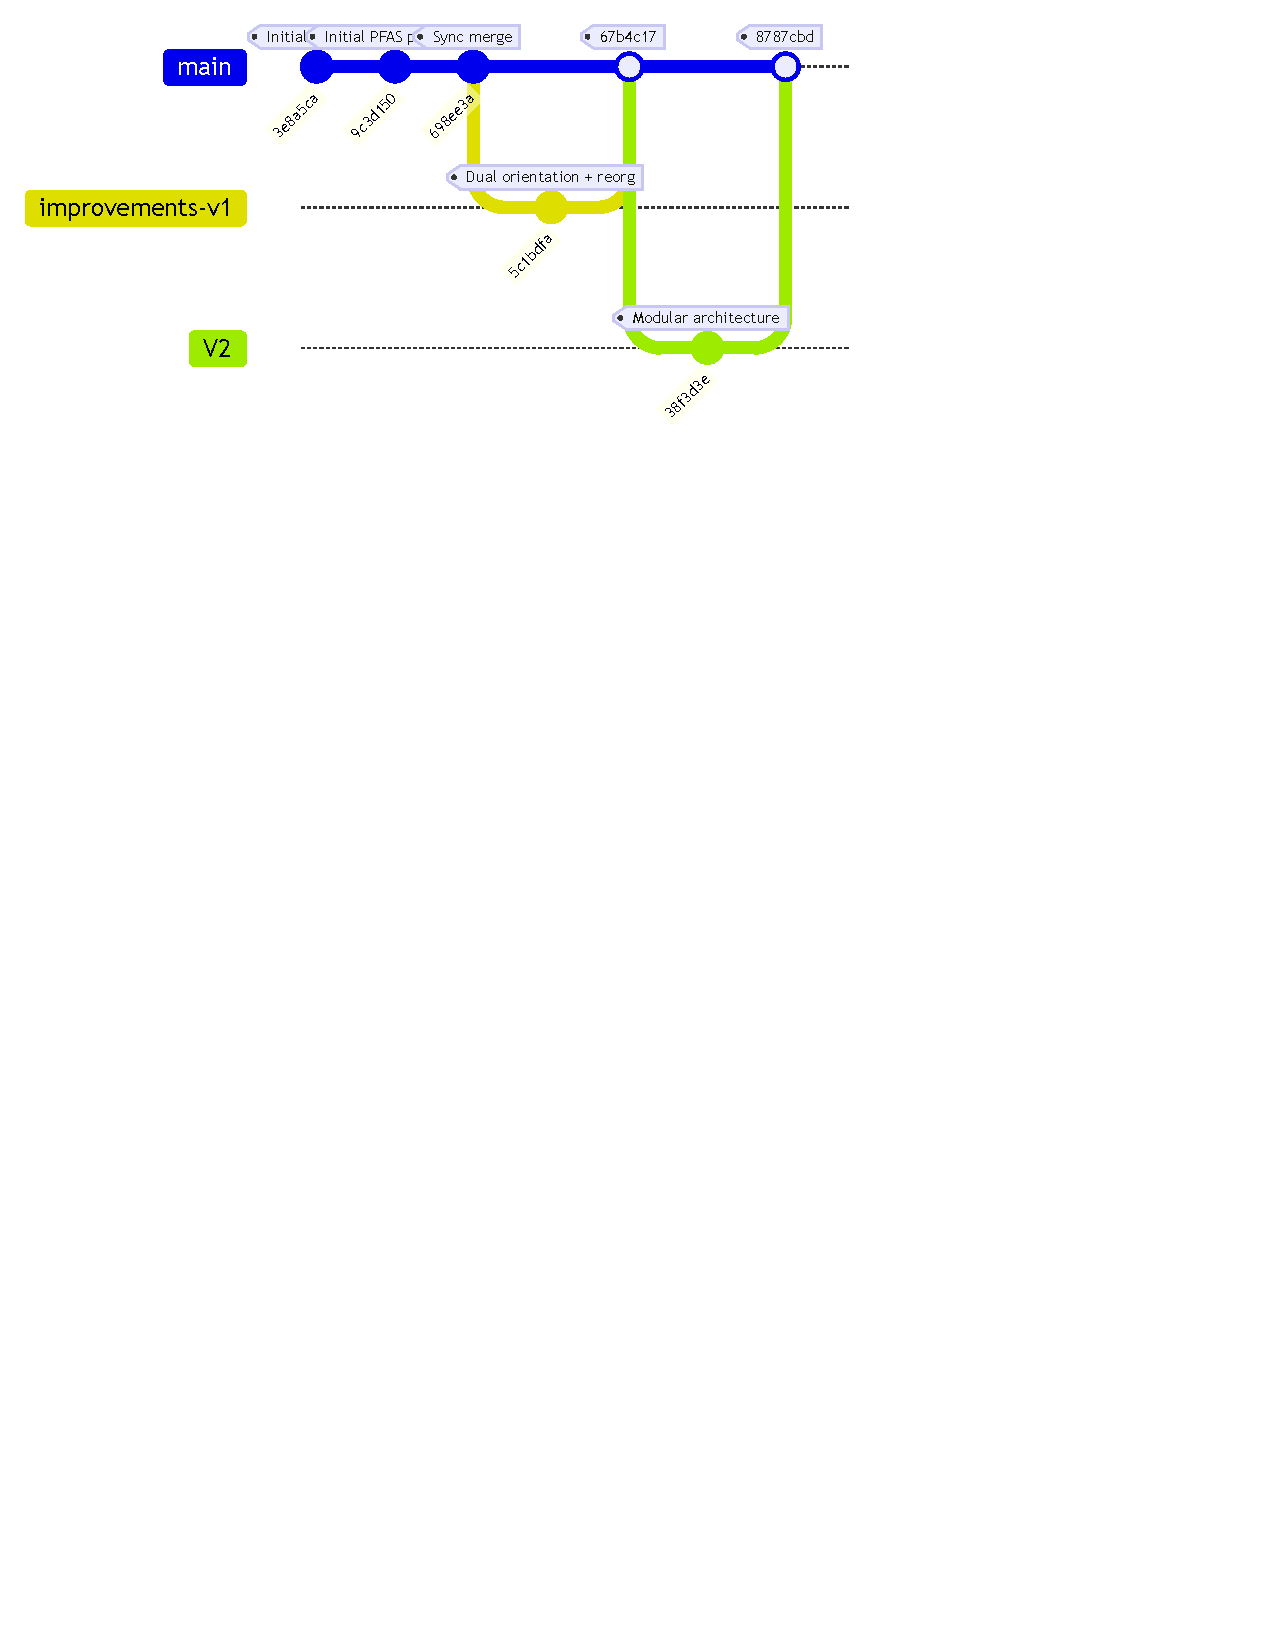
\includegraphics[width=\textwidth,height=0.75\textheight,keepaspectratio]{git_history.pdf}
\caption{Repository branch and merge evolution (Mermaid gitGraph rendered to PDF).}
\end{figure}

\subsection{Impact of the Two Major Refactors}
\textbf{Refactor 1 (\texttt{5c1bdfa}):}
\begin{itemize}[leftmargin=1.5em]
\item Brought dual-orientation execution into the main production path.
\item Introduced cleaner repository layout and retained manuscript within \texttt{docs/}.
\item Established stronger CLI usage patterns for single molecule and batch directory runs.
\end{itemize}

\textbf{Refactor 2 (\texttt{38f3d3e}):}
\begin{itemize}[leftmargin=1.5em]
\item Split monolithic script into composable modules.
\item Improved maintainability and testability by separating geometry/math, orchestration, analysis, and reporting.
\item Kept backward compatibility through \texttt{run\_pfas\_interface\_knf.py} shim.
\end{itemize}

\section{End-to-End Computational Workflow}
\subsection{Operational Pipeline}
\begin{figure}[H]
\centering
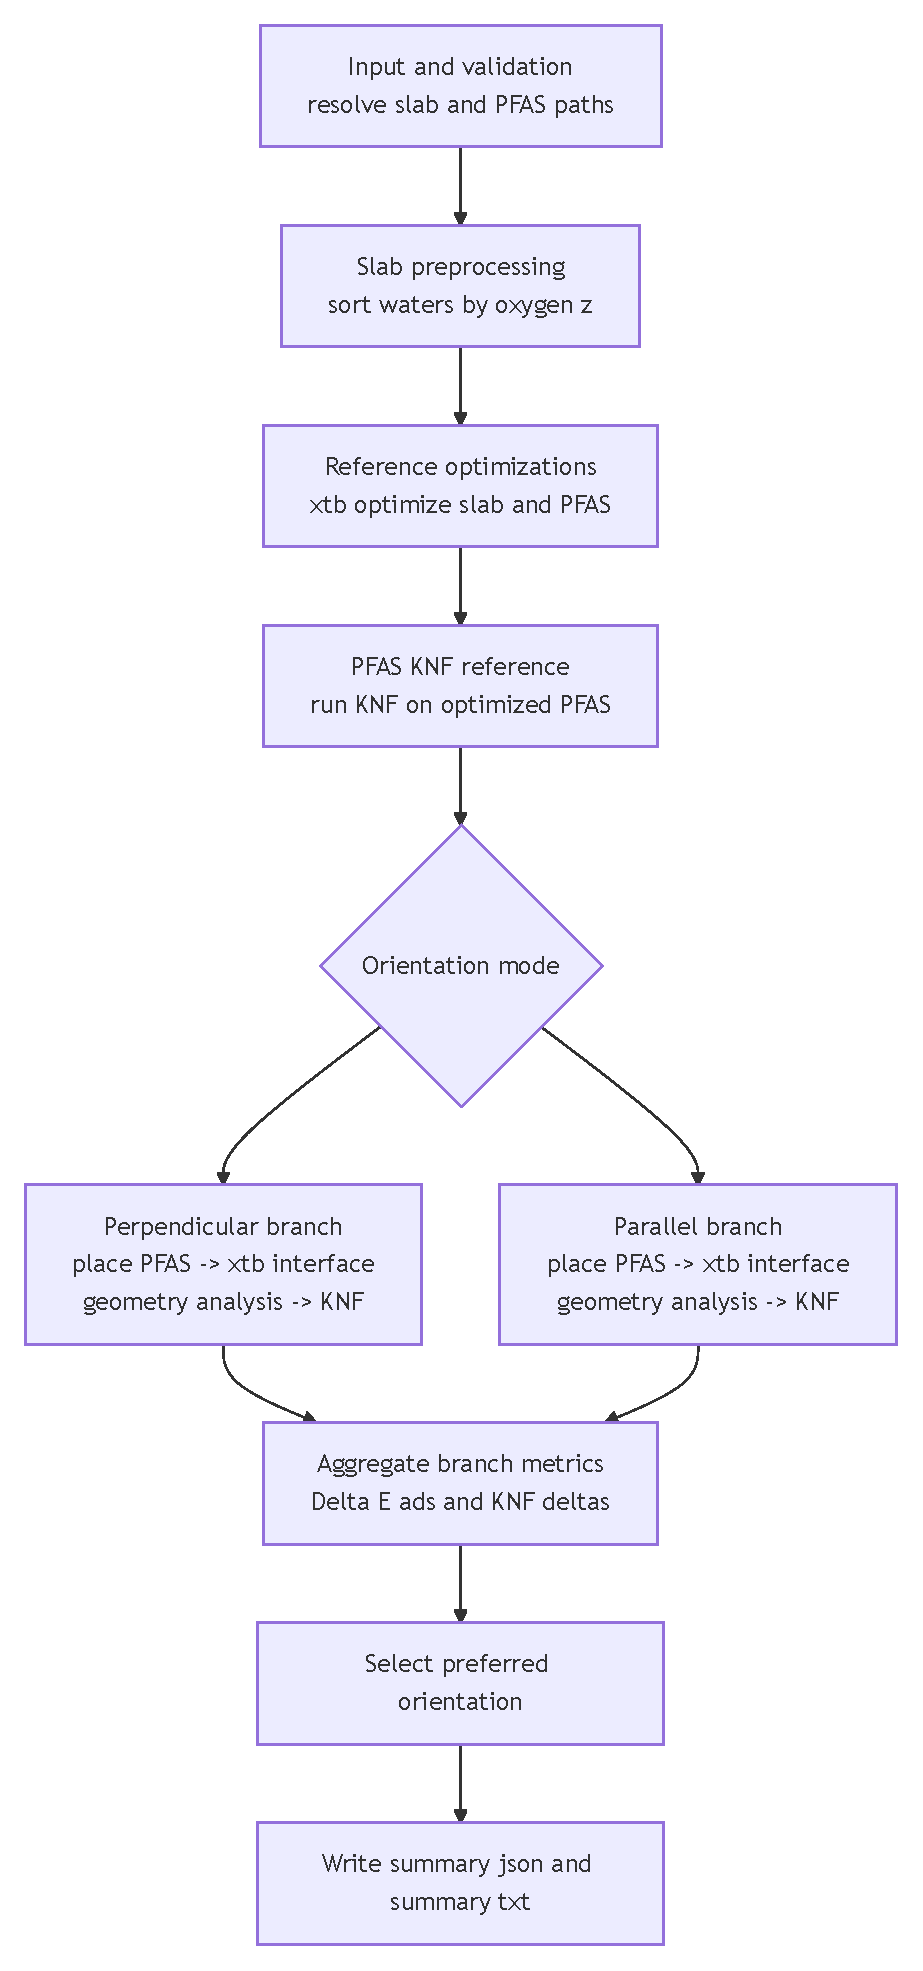
\includegraphics[width=\textwidth,height=0.75\textheight,keepaspectratio]{workflow_overview.pdf}
\caption{Production workflow from input ingestion to orientation selection and final summaries.}
\end{figure}

\subsection{Step-by-Step Execution}
For each PFAS molecule, workflow execution in \texttt{workflow.py} is:
\begin{enumerate}[leftmargin=1.5em]
\item Validate slab and PFAS inputs.
\item Create deterministic run directory and step subfolders.
\item Sort slab waters by oxygen z-order (expects O-H-H triplets).
\item xTB optimize slab.
\item xTB optimize PFAS.
\item Run KNF on optimized PFAS (gas-like context used by current workflow).
\item For each orientation branch (perpendicular, parallel):
\begin{itemize}[leftmargin=1.5em]
\item infer axis, rotate and place PFAS above slab,
\item optimize interface with xTB,
\item run geometry diagnostics,
\item run KNF on optimized interface,
\item compute KNF metric shifts versus PFAS reference.
\end{itemize}
\item Compute adsorption energy for each branch and pick preferred orientation by minimum \(\Delta E_{ads}\).
\item Emit machine-readable \texttt{summary.json} and human-readable \texttt{summary.txt}.
\end{enumerate}

\subsection{Run Directory Contract}
\begin{figure}[H]
\centering
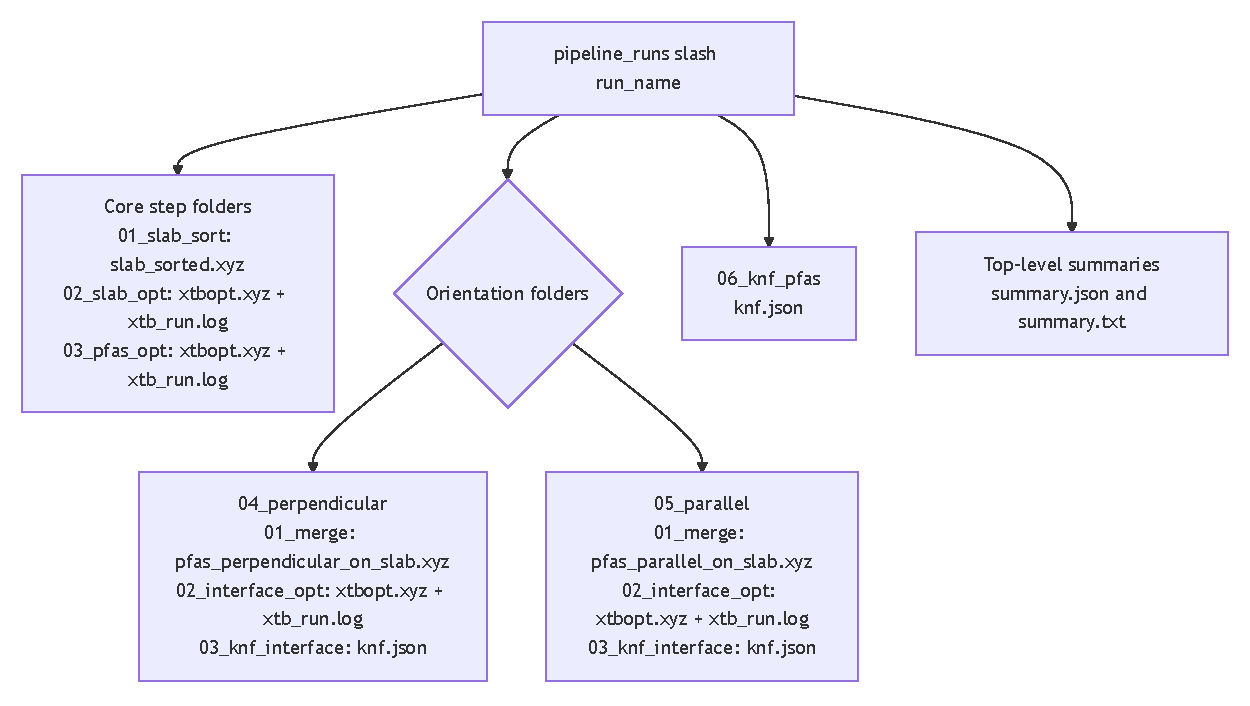
\includegraphics[width=\textwidth,height=0.75\textheight,keepaspectratio]{run_directory_layout.pdf}
\caption{Expected per-run artifact layout and orientation branch output structure.}
\end{figure}

\section{Mathematical and Methodological Core}
\subsection{Placement Transform}
PFAS placement above slab is computed by translation:
\begin{align}
\Delta x &= x^{center}_{slab} - x^{ref}_{pfas} + x_{shift}, \\
\Delta y &= y^{center}_{slab} - y^{ref}_{pfas} + y_{shift}, \\
\Delta z &= (z^{max}_{slab} + g) - z^{anchor}_{pfas}.
\end{align}

Current production default in \texttt{workflow.py} is \(g = \SI{1.5}{\angstrom}\).

\subsection{Energy Definitions}
The workflow uses standard adsorption decomposition:
\begin{equation}
\Delta E_{ads,o} = E_{interface,o} - E_{slab} - E_{PFAS}, \quad o \in \{\perp,\parallel\}
\end{equation}

Orientation anisotropy:
\begin{equation}
\Delta\Delta E = \Delta E_{\parallel} - \Delta E_{\perp}
\end{equation}

Interpretation:
\begin{itemize}[leftmargin=1.5em]
\item \(\Delta\Delta E > 0\): perpendicular favored.
\item \(\Delta\Delta E < 0\): parallel favored.
\item \(|\Delta\Delta E| \lesssim \SI{15}{kJ\,mol^{-1}}\): orientation-indifferent zone (manuscript criterion).
\end{itemize}

\subsection{KNF Context and Descriptor Flow}
\begin{figure}[H]
\centering
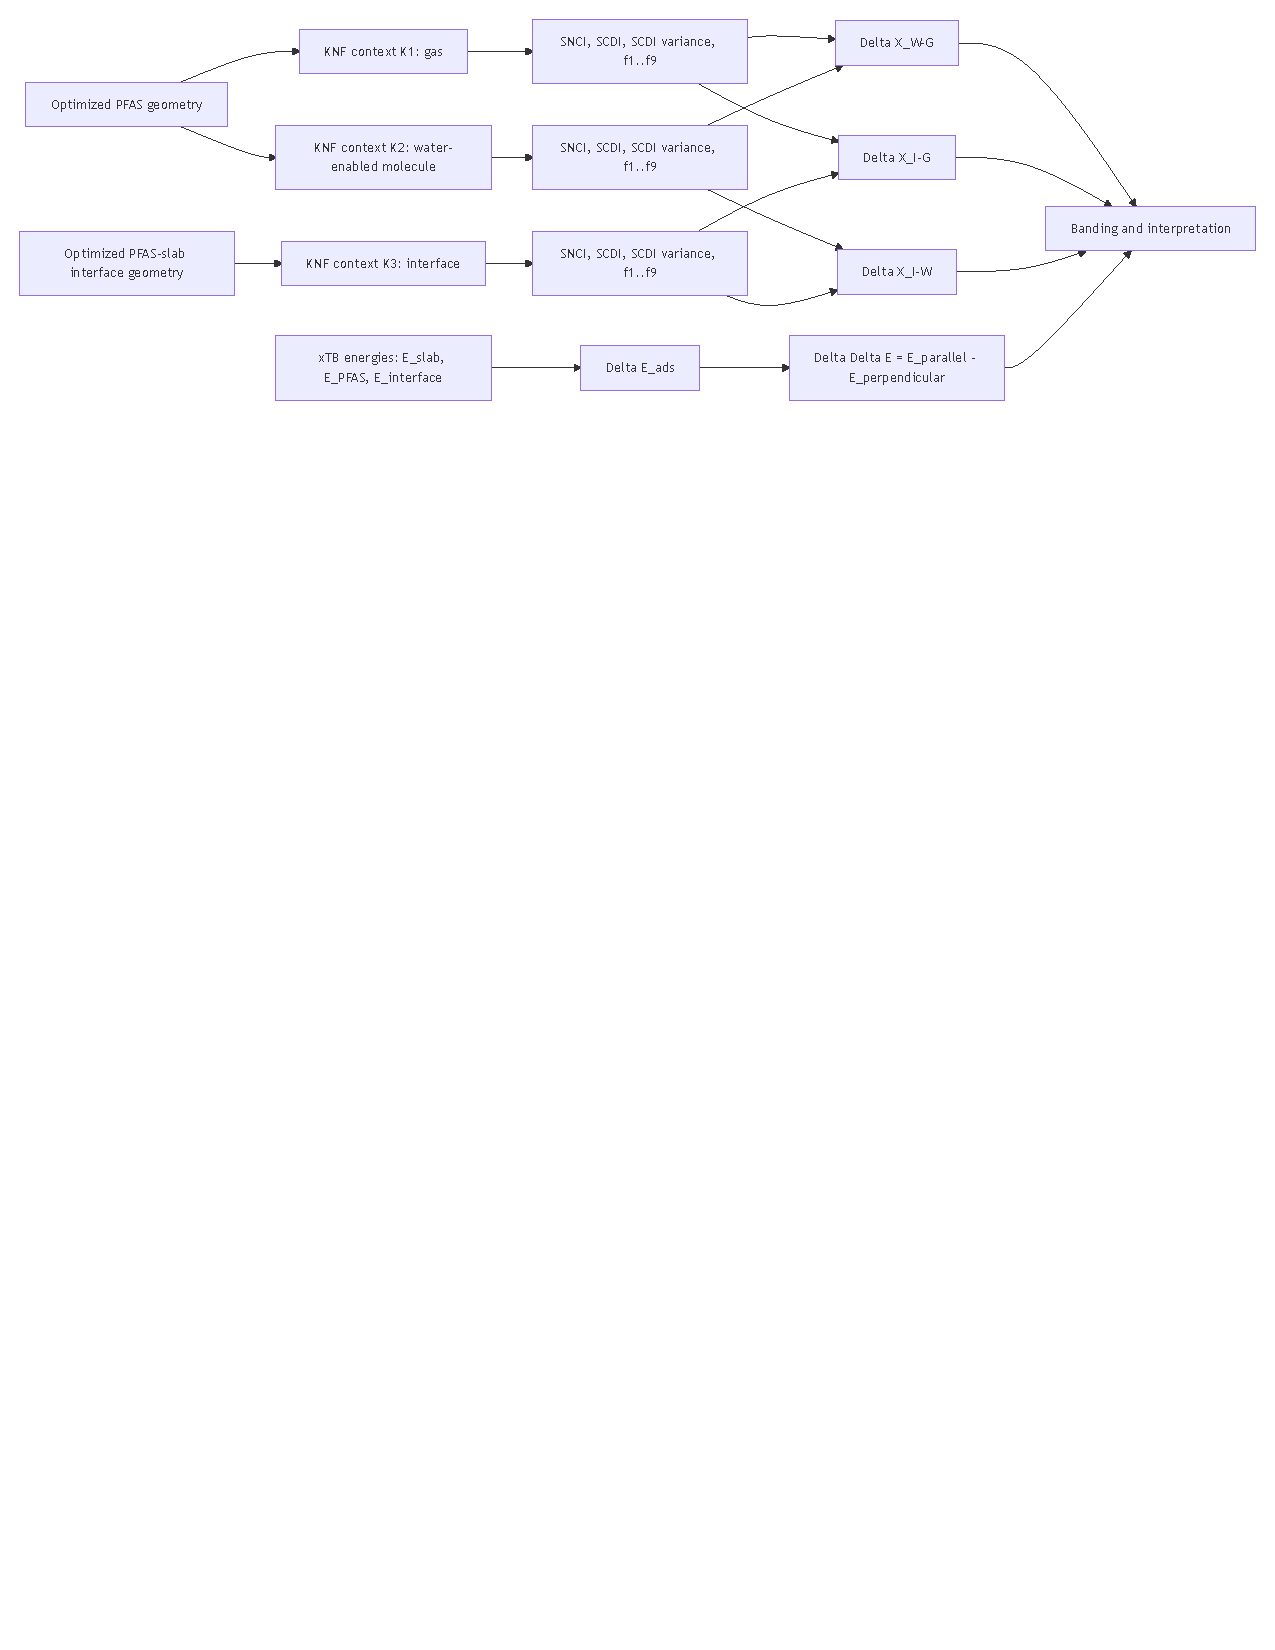
\includegraphics[width=\textwidth,height=0.75\textheight,keepaspectratio]{descriptor_pipeline.pdf}
\caption{Descriptor pathway from xTB structures to KNF vectors/scalars and delta features.}
\end{figure}

Manuscript methodology defines three KNF contexts (gas, water-enabled molecule, interface). Current code computes PFAS and interface KNF in pipeline form and stores KNF vector/scalar outputs for shift analysis.

\section{CLI Interfaces and Arguments}
\subsection{Primary Commands}
\begin{itemize}[leftmargin=1.5em]
\item \texttt{PFAS <input\_file\_or\_directory>} (user-facing production command)
\item \texttt{pfas-interface-knf <slab.xyz> <pfas.xyz>} (explicit workflow command)
\end{itemize}

\subsection{Argument Layers}
\textbf{Essential layer (typical user path):}
\begin{itemize}[leftmargin=1.5em]
\item input PFAS file or directory,
\item optional \texttt{--slab},
\item optional \texttt{--pfas-charge}.
\end{itemize}

\textbf{Advanced layer (reproducibility and sweeps):}
\begin{itemize}[leftmargin=1.5em]
\item \texttt{--run-root}, \texttt{--run-name}
\item \texttt{--gap}, \texttt{--x-shift}, \texttt{--y-shift}
\item \texttt{--orientation-mode}\; (\texttt{dual|perpendicular|parallel})
\item \texttt{--multiplicity}, \texttt{--gfn}
\item \texttt{--contact-elements}
\item \texttt{--keep-knf-intermediates}
\item \texttt{--knf-scdi-var-min}, \texttt{--knf-scdi-var-max}
\end{itemize}

\subsection{Observed Default Mismatch (Important)}
Current code has a noteworthy mismatch:
\begin{itemize}[leftmargin=1.5em]
\item \texttt{workflow.py} default \texttt{--gap} = \texttt{1.5}
\item \texttt{cli.py} default \texttt{--gap} = \texttt{2.5}
\end{itemize}
For strict reproducibility, pass \texttt{--gap} explicitly until these defaults are unified.

\section{Mapping to Manuscript Methodology}
\subsection{Directly Implemented in Repository}
\begin{itemize}[leftmargin=1.5em]
\item Dual-orientation branch generation (perpendicular and parallel).
\item xTB optimization of slab, PFAS, and each interface branch.
\item Adsorption-energy decomposition and orientation selection.
\item Geometry diagnostics (z-extents, contact distance, placement class logic).
\item KNF post-processing on optimized PFAS and optimized interface geometries.
\end{itemize}

\subsection{Manuscript Details Referenced in This Report}
Values used from \texttt{docs/manuscript.pdf} include:
\begin{itemize}[leftmargin=1.5em]
\item Dataset size and diversity: 88 compounds across 15 families.
\item Canonical slab model: 96 waters (288 atoms), area \SI{12.72}{\angstrom} x \SI{11.64}{\angstrom}, thickness \SI{19.03}{\angstrom}, apparent density 1.018 g cm\textsuperscript{-3}.
\item Five-band SNCI framework: Band I (<800), II (800--830), III (830--860), IV (860--890), V (>890).
\item Reported orientation anisotropy range: \SI{-447.3}{kJ\,mol^{-1}} to \SI{216.8}{kJ\,mol^{-1}}.
\end{itemize}

\section{Sample Calculations (Manuscript-Aligned)}
\subsection{Energy Unit Conversion}
Manuscript uses \(1\,\mathrm{Eh} = 2625.5\,\mathrm{kJ\,mol^{-1}}\). Converting representative \(\Delta\Delta E\):
\begin{align}
\Delta\Delta E_{PFOA} &= +6.7\,\mathrm{kJ\,mol^{-1}} = +0.002552\,\mathrm{Eh} \\
\Delta\Delta E_{PFOS} &= +216.8\,\mathrm{kJ\,mol^{-1}} = +0.082575\,\mathrm{Eh} \\
\Delta\Delta E_{PIN04} &= -447.3\,\mathrm{kJ\,mol^{-1}} = -0.170368\,\mathrm{Eh}
\end{align}

\subsection{Orientation Interpretation Examples}
\begin{table}[H]
\centering
\caption{Representative orientation interpretation using manuscript values}
\begin{tabular}{p{0.22\textwidth}p{0.20\textwidth}p{0.52\textwidth}}
\toprule
Compound & Reported \(\Delta\Delta E\) & Interpretation \\
\midrule
PFOA & +6.7 kJ mol\textsuperscript{-1} & Orientation-indifferent regime (close energetic competition between parallel and perpendicular). \\
PFOS & +216.8 kJ mol\textsuperscript{-1} & Strong perpendicular preference; high anisotropy and robust orientation lock. \\
PIN04 & -447.3 kJ mol\textsuperscript{-1} & Extreme parallel preference; orientation dominated by strong branch asymmetry. \\
\bottomrule
\end{tabular}
\end{table}

\section{Known Limitations and Risk Register}
\begin{table}[H]
\centering
\caption{Current limitations relevant to reproducibility and scale-up}
\begin{tabular}{p{0.23\textwidth}p{0.33\textwidth}p{0.36\textwidth}}
\toprule
Area & Current limitation & Practical impact \\
\midrule
Defaults consistency & \texttt{--gap} mismatch between \texttt{cli.py} and \texttt{workflow.py}. & Runs launched through different entry points may not match unless \texttt{--gap} is explicit. \\
Input assumptions & Slab sorter requires strict O-H-H ordering and atom count divisible by 3. & Non-canonical slab files can fail early. \\
xTB dependency & Requires external \texttt{xtb} executable in \texttt{PATH}. & Environment setup failure blocks all optimization stages. \\
KNF dependency & Requires functioning \texttt{knf\_core.pipeline}. & KNF stage unavailable if local KNF environment is broken. \\
Error resilience & No full batch resume database in current CLI path. & Interrupted large campaigns may need partial reruns depending on run state. \\
Finite slab geometry & Canonical finite slab can underrepresent long-chain lateral contact in some parallel poses (manuscript-noted). & Potential bias for very long PFAS in edge placement configurations. \\
\bottomrule
\end{tabular}
\end{table}

\section{Operational Reproduction Guide}
\subsection{Environment Prerequisites}
\begin{itemize}[leftmargin=1.5em]
\item Python >= 3.10
\item xTB executable available on \texttt{PATH}
\item KNF package installed and importable (\texttt{knf\_core.pipeline})
\item This repository installed in editable mode:
\end{itemize}

\begin{verbatim}
python -m pip install -e .
\end{verbatim}

\subsection{Single-Molecule Production Run}
\begin{verbatim}
PFAS .\molecules\PFOA.xyz --pfas-charge -1 --gap 1.5 --orientation-mode dual
\end{verbatim}

\subsection{Batch Directory Run}
\begin{verbatim}
PFAS .\molecules --pfas-charge -1 --gap 1.5 --run-root .\pipeline_runs
\end{verbatim}

\subsection{Expected Primary Outputs}
\begin{itemize}[leftmargin=1.5em]
\item \texttt{summary.json}: full machine-readable run payload
\item \texttt{summary.txt}: human-readable report
\item Orientation-specific interface \texttt{xtbopt.xyz} and \texttt{knf.json}
\item PFAS KNF reference \texttt{knf.json}
\end{itemize}

\section{Conclusion}
The repository has evolved from a strong proof-of-concept monolith into a modular production-ready workflow with clear separation of concerns. It already encodes the critical dual-orientation interfacial methodology, xTB/KNF coupling, and report-generation path needed to reproduce the study logic in \texttt{docs/manuscript.pdf}. The immediate path to highly reliable re-production is to standardize defaults (especially gap), add explicit batch resume bookkeeping, and add test coverage around slab parsing, orientation transforms, and summary schema stability.

\section*{Primary Internal Sources}
\begin{itemize}[leftmargin=1.5em]
\item Repository history: \texttt{git log} up to \texttt{8787cbd}
\item Code modules under \texttt{pfas\_interface\_cli/}
\item Manuscript: \texttt{docs/manuscript.pdf}
\end{itemize}

\end{document}





